\section{Introduction}
\begin{frame}
\frametitle{Introduction}
We can derive the mathematical model of a system in two ways mainly:
\begin{itemize}
	\item Physical Modeling: 
	
	Applying the laws of physics, chemistry, thermodynamics,...
	Also called modeling from \emph{First Principles}
	
	\pause 
	
	\item  System identification or \emph{Empirical Modeling}:
	
	Developing models from observed or collected data
	\begin{figure}
	\centering
	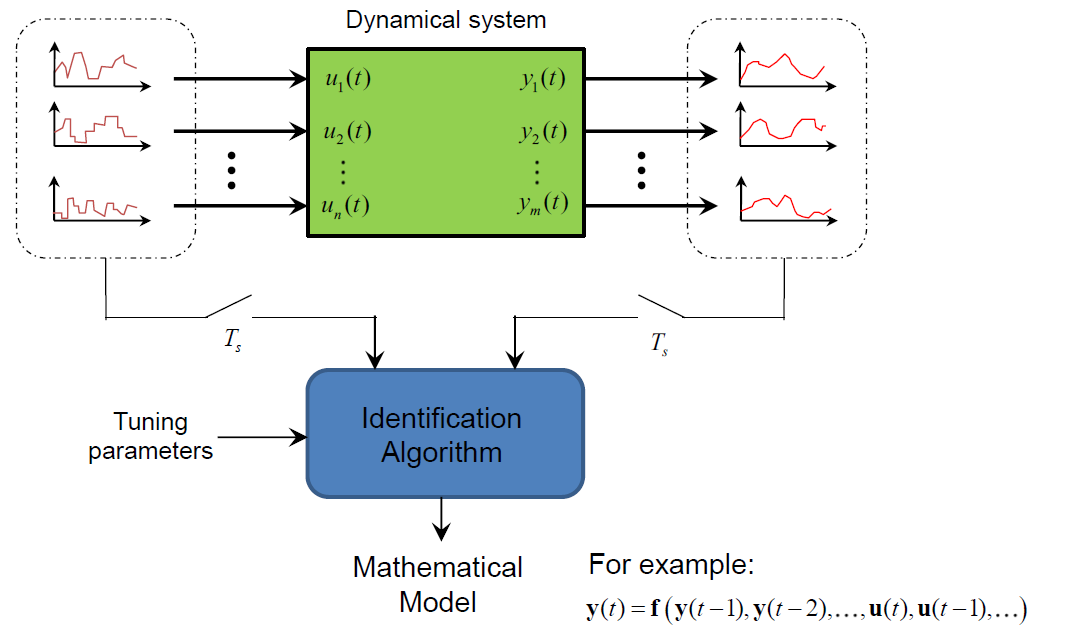
\includegraphics[width=0.7\linewidth]{img/system-identification}
	%\caption{}
	\label{fig:system-identification}
	\end{figure}

\end{itemize}
\end{frame}


\section{First Principles Modeling}

% Counter for the example numbers
\newcounter{exampleCount}

\begin{frame}
	\stepcounter{exampleCount}
	\frametitle{Example \arabic{exampleCount}: Mass-Spring System} 
	
	\begin{columns}
		\begin{column}{0.4\linewidth}
			\begin{figure}
			\centering
			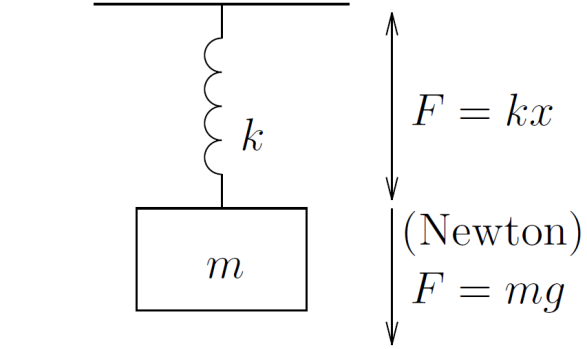
\includegraphics[width=1\linewidth]{img/mass-spring}
			\label{fig:mass-spring}
			\end{figure}
		\end{column}
		\begin{column}{0.6\linewidth}
			If spring is at rest at $x=0$:
			\begin{align*}
			m \cdot \frac{d^{2}x}{dt^{2}} + k \cdot x =  m \cdot g \\
			\end{align*}
		\end{column}
	\end{columns}
\end{frame}


\begin{frame}
	\stepcounter{exampleCount}
	\frametitle{Example \arabic{exampleCount}: Mass-Spring Damped}
	\begin{figure}
\centering
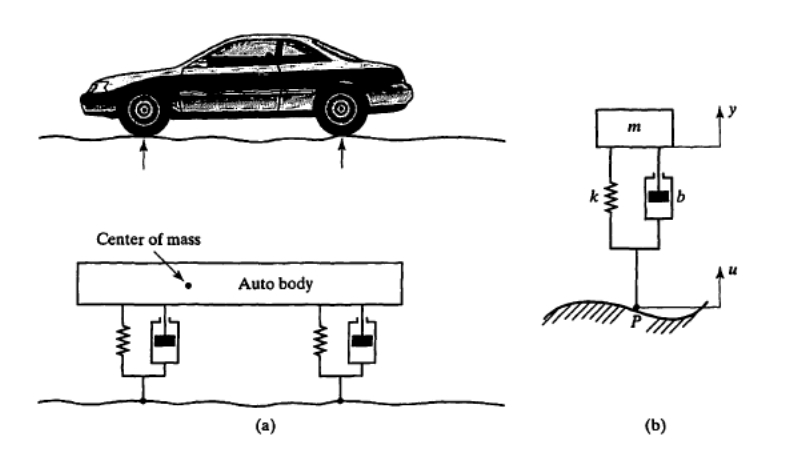
\includegraphics[width=1\linewidth]{img/mass-spring-damped}
\label{fig:mass-spring-damped}
\end{figure}
\emph{\textcolor{blue}{ \href{https://youtu.be/8DuJEpy-ODo}{Animation} }}
\end{frame}

\begin{frame}
	\stepcounter{exampleCount}
	\frametitle{Example \arabic{exampleCount}: Pendulum}
	\begin{columns}
		 \begin{column}{0.5\linewidth}
		 	\begin{figure}
			\centering
			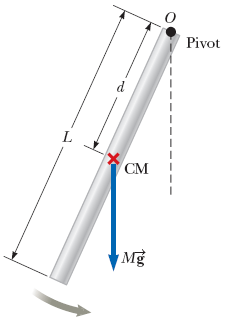
\includegraphics[width=0.9\linewidth]{img/pendulum}
			\label{fig:pendulum}
			\end{figure}
		 \end{column}
		 \begin{column}{0.5\linewidth}
		 	todo
		 \end{column}
	\end{columns}
\end{frame}

\begin{frame}
	\stepcounter{exampleCount}
	\frametitle{Example \arabic{exampleCount}: Inverted Pendulum}
	\begin{figure}
	\centering
	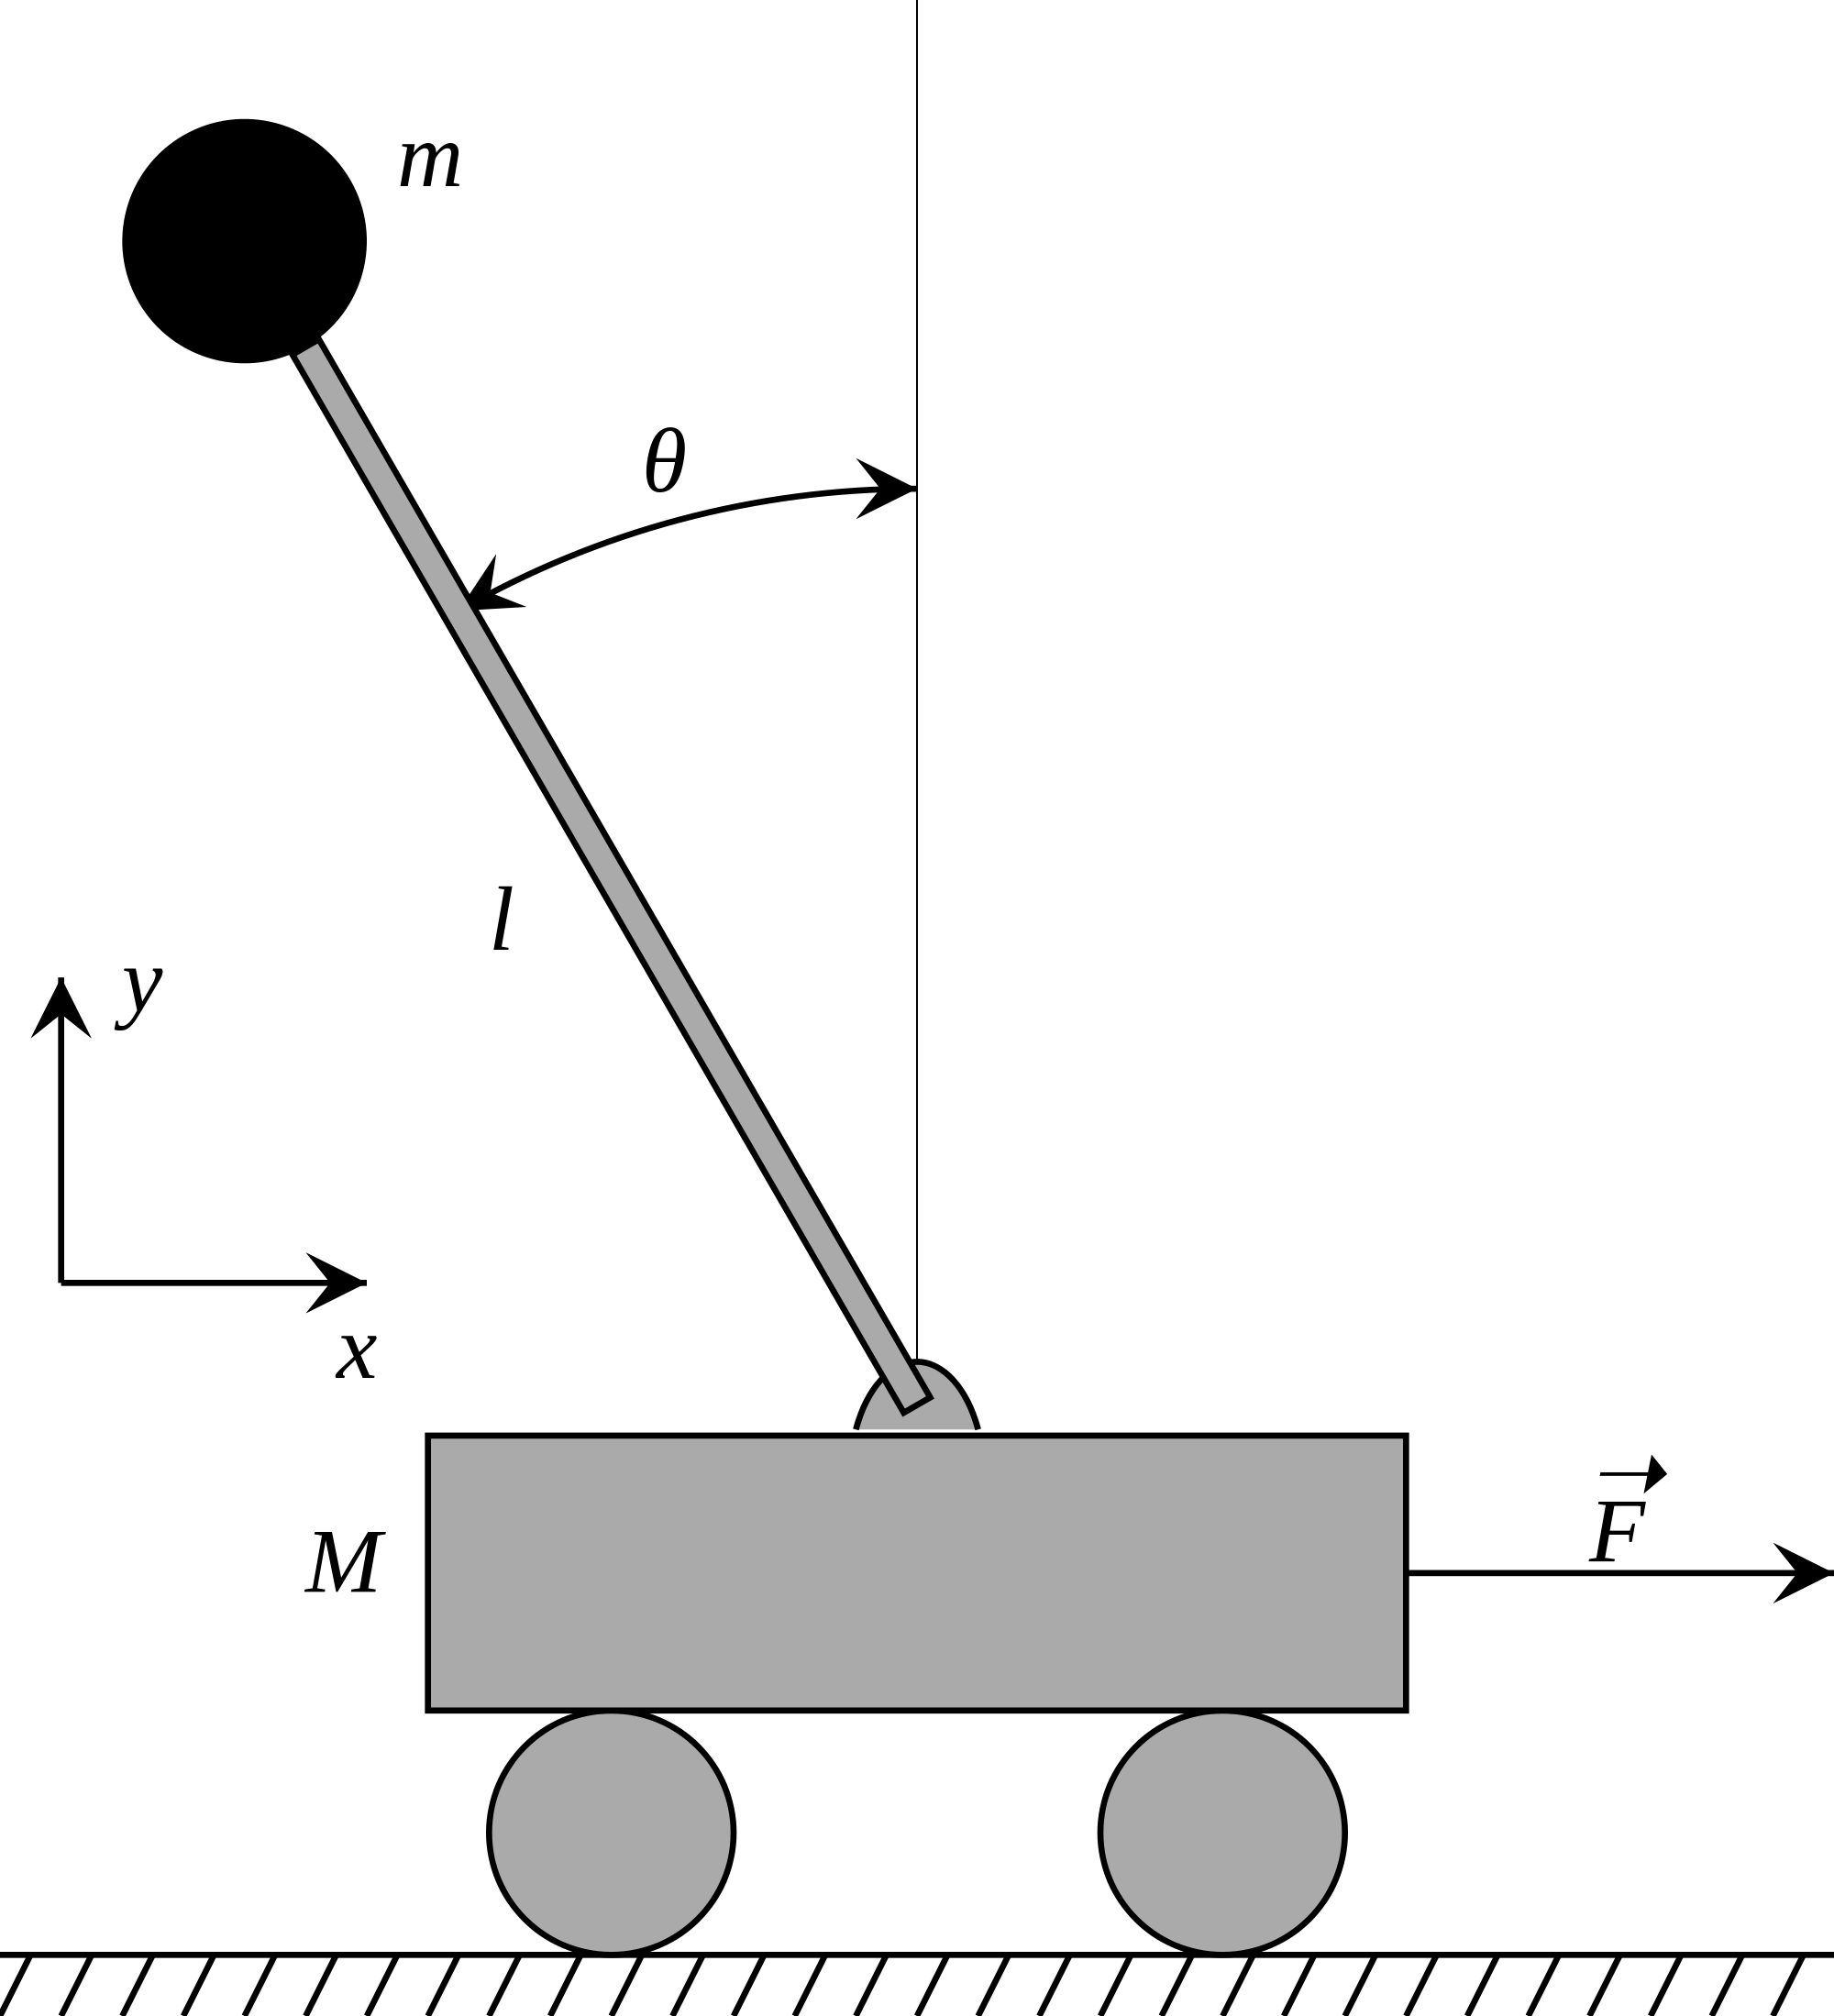
\includegraphics[width=0.6\linewidth]{img/pendulum-inverted}
	\label{fig:pendulum-inverted}
	%youtube: https://www.youtube.com/watch?v=15DIidigArA
	\end{figure}
\end{frame}

\begin{frame}
	\stepcounter{exampleCount}
	\frametitle{Example \arabic{exampleCount}: RLC Circuit}
	
		\begin{figure}
		\centering
		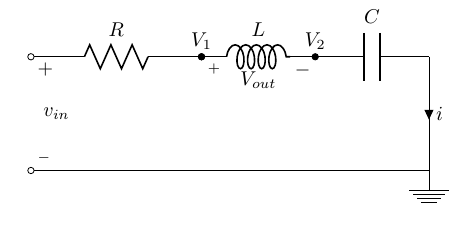
\includegraphics[width=0.7\linewidth]{img/circuit-RLC}
		\label{fig:circuit-RLC}
		\end{figure}
		Besides input $v_{in}$, two internal variables needed to determine output $\Rightarrow$ Second-order System
		\begin{center}
			\begin{tabular}{c@{\hskip 1cm} c@{\hskip 1cm} c}
				Inputs 	& Ouputs 	& Choosen States \\ \hline
				$v_{in}$ 	& $v_{out}$	& $V_2$ \\
				& & $i$ \\ 
			\end{tabular}
		\end{center}
		
\end{frame}

\begin{frame}
	\stepcounter{exampleCount}
	\frametitle{Example \arabic{exampleCount}: RLC Circuit}
	
	\begin{columns}
		\begin{column}{0.4\linewidth}
			Equations for each component:
			\begin{align*}
			&i = \frac{V_{in} - V_{1}}{R} \\
			&V_1 - V_2 = L \cdot \frac{di}{dt} \\
			&i = C \cdot \frac{dV_2}{dt} \\
			\end{align*}
		\end{column}
		\begin{column}{0.6\linewidth}
			\begin{figure}
				\centering
				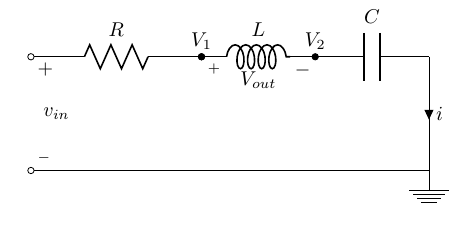
\includegraphics[width=1\linewidth]{img/circuit-RLC}
				\label{fig:circuit-RLC-small}
			\end{figure}
		\end{column}
		
	\end{columns}
	
\end{frame}
\begin{frame}
	\stepcounter{exampleCount}
	\frametitle{Example \arabic{exampleCount}: RLC Circuit}
	\begin{itemize}
		\item Writing derivatives of state variables in function of state variables and inputs:
		
		\item Writing output in function of state variables and inputs:
	\end{itemize}
	\begin{block}{State Space Representation}
		This yields the State Space Representation of the dynamic system. In Matrix form:
		\begin{align*}
			\begin{bmatrix}
			a & b 
			\end{bmatrix}
		\end{align*}
	\end{block}
			
\end{frame}
